\chapter{Modeling bound-state diffusion in selective filters}\label{ch02}

%Selective filters made of biopolymers are used in living and
%synthetic systems to control the localization and movement of
%molecules, nanoparticles, viruses and other organisms \cite{witten17}.
%These filters regulate access to genetic material (the nuclear pore
%complex, or NPC), cells (the pericellular matrix), tissues (the
%extracellular matrix), and organs (mucus). In addition to their
%protective role, polymeric biomaterials are physical barriers that can
%inhibit drug delivery. Microbial biofilms can sequester antibiotics in
%their pericellular matrix, hindering treatment of infections
%\cite{hoiby10}. The extracellular matrix and mucosal layers limit drug
%delivery in cancer and other diseases \cite{witten17}. How particle
%binding affects motion and filtering is unclear. Binding to the
%pericellular matrix facilitates uptake of nanoparticles by single
%cells \cite{zhou12}, and transport factors that bind to proteins in
%the NPC move rapidly through it \cite{strambio-de-castillia10}.  In
%contrast, binding inhibits the uptake of nanoparticles that bind to
%airway mucus \cite{schneider17, huang17, mastorakos15}. Many viruses
%minimize binding interactions, allowing human papillomavirus and human
%immunodifficiency virus to move nearly unrestricted in cervical mucus
%under certain conditions \cite{olmsted01,lai09}, although antibody binding 
%can slow these interactions \cite{chen14}.  Improved design of
%drug delivery vehicles and synthetic selective filters requires
%understanding what distinguishes these behaviors.  While particle
%size, charge, and binding interactions are known to affect filtering
%\cite{witten17}, the physical principles that underlie mobility and
%transport in polymeric biomaterials are not fully understood.
%
%Among these filters, the NPC is tuned for selective passage enabled by
%binding.  The NPC selectively filters molecular traffic between the
%nucleus and cytoplasm of eukaryotic cells, making it important for
%diverse processes including gene regulation and translation
%\cite{strambio-de-castillia10}. Transport occurs through the central
%channel, $\sim$50 nm in diameter and $\sim$100 nm long. The selective
%barrier filling the central channel is made from disordered proteins,
%the FG nucleoporins (FG Nups), which contain repeated
%phenylalanine-glycine (FG) motifs \figref{fig:cartoon}.  Transport
%factors (TFs) that directly bind to the FG repeats can cross the NPC
%and carry cargo with them \cite{strambio-de-castillia10}.  Transport
%through the NPC is remarkably fast, with pore residence times $\sim$10
%ms \cite{yang04}.  Binding between FG Nups and TFs shows
%diffusion-limited on-rates and transient binding of individual FG
%repeats to TFs \cite{milles15, hough15}.  How the FG Nups both block
%passage (of non-binding molecules) and facilitate passage (of binding
%molecules) is not fully understood, making the NPC an ideal system to
%dissect the principles of binding-controlled selective transport.

%Models of the NPC selective barrier have proposed that the FG Nups may
%form an entropic brush \cite{rout00}, a dynamic hydrogel
%\cite{ribbeck01, frey07}, an intermediate state between a brush and
%gel \cite{vovk16}, or liquid droplets \cite{schmidt15}.  These
%mechanisms may be modulated by spatial organization \cite{yamada10,
%  ando14} and binding of TFs to multiple FG repeats \cite{lowe15,
%  schoch12}.  Attempts to distinguish these models have been hindered
%by the pore's small size, the redundancy and multiple copies of FG
%Nups, and contradictory experimental results on FG Nups and TF binding
%\cite{vovk16}. Some FG Nup fragments form less-dynamic hydrogels
%\vitro\ \cite{frey07}, but remain highly dynamic within cells
%\cite{hough15}. Molecular dynamics simulations find highly dynamic FG
%Nups, though the degree and extent of motion depends on the affinity
%of FG repeats for each other and for TFs \cite{pulupa17,
%  vovk16}. Crowding and competition modulate affinity
%\cite{tetenbaum-novatt10} and may contribute to selective transport
%\cite{zilman07}.  However, the connection between the amino-acid level
%behavior of the FG-TF interaction and macroscopic transport
%selectivity remains unclear.  Here we address the central
%contradiction of selective transport through the NPC: how does binding
%of TFs to FG Nups within the pore increase the flux rather than
%decreasing it \cite{bickel02, witten17}?
%
%Using a biophysical model, we demonstrate that TF diffusion and
%binding are sufficient for selective transport, as long as binding
%only partially immobilizes TFs. Binding increases the local
%concentration, and these molecules contribute to the flux if mobile.
%Thermally-driven diffusion of TFs bound to flexible tethers gives
%sufficient particle mobility to produce selectivity similar to
%experimental measurements.  Tether flexibility also allows bound TFs
%to hop between tethers, further enhancing selectivity.
%
%We consider a minimal model of the central channel of the NPC
%containing FG Nups homogeneously anchored \figref{fig:cartoon}.  This
%model is sufficiently general to describe the common features of a
%range of biopolymer filters.   A varying free energy landscape
%along the axis of the NPC may play a role in selective transport
%\cite{zilman07, tagliazucchi13, tu13, timney16}.

The nuclear pore is a clear example of a selective biofilter, but the precise mechanism of selectivity is not well understood.  In particular, an apparent paradox arises from the fact that transport factors, which bind to FG Nups within the pore, have a much higher flux through the pore than inert, nonbinding proteins.  This result is somewhat counterintuitive, given that binding must necessarily slow the passage of a transport factor through the pore.  In addition to nuclear transport, binding and diffusion are important in many other biofilters as well, including drug delivery through a mucus layer liquid-liquid phase separation (Sec.~\ref{sec:other-filters}) \cite{schneider17, huang17, mastorakos15,brangwynne15, feric16,witten17}.  We wanted to understand how binding increases flux through selective biofilters.

To that end, we developed a simple mathematical model of selective transport inspired by the nuclear pore.  While the model is based on nuclear transport, it is general enough that it can be applied to a wide range of biological systems and synthetic biofilters.  Unlike most existing theoretical models of nuclear transport, which reduce transport to diffusion in a single effective one-dimensional potential, this model does not require simulations or a precise accounting of the locations and composition of Nups along the pore axis \cite{pulupa17, vovk16,tagliazucchi13, tu13, timney16}.  It is equally applicable to a bulk material as to a nanopore.  A few other first-principles models of the pore have been developed using similar differential equations but making different assumptions about boundary conditions and binding equilibrium \cite{zilman07,yang18}.

The primary surprising result of our model was the importance of bound-state diffusion for selectivity.  No selective filtering was possible if the transport factor - Nup complex was immobile, regardless of the other parameters.  However, if bound diffusion within the pore was permitted, the selective flux of transport factor through the pore as compared to that of an inert protein approached that measured experimentally.  These results suggest that bound-state diffusion is key to selective transport within the nuclear pore and perhaps to a number of other biofilters as well.

The work in this chapter was a close collaboration between myself, Mike Stefferson, and Loren Hough.  Mike contributed significantly to developing the model and wrote the numerical simulations in both the linear and non-linear cases.

\section{Simplified model of nuclear transport}
\label{sec:model}

Nuclear transport is highly complex, but its unusual selective properties can be modeled much more simply than can the entirety of transport.  A major goal of our model was to reproduce the selectivity of the nuclear pore in most straightforward way possible.  To that end, we made many simplifying assumptions.  The nuclear pore was treated as a one-dimensional selective membrane uniformly filled with Nups.  While the nuclear pore itself has a non-uniform, asymmetric distribution of Nups along its axis, as well as variation in the FG motif density along its radius, its selectivity remains intact when the asymmetric Nups are removed.  In fact, a significant fraction of Nups can be removed without destroying selectivity \cite{strawn04, zeitler04,kowalczyk11, jovanovic-talisman09}.  Any possible wide capture area outside the pore is also neglected \cite{pagliara14}.

\begin{figure}[t!]
\centering
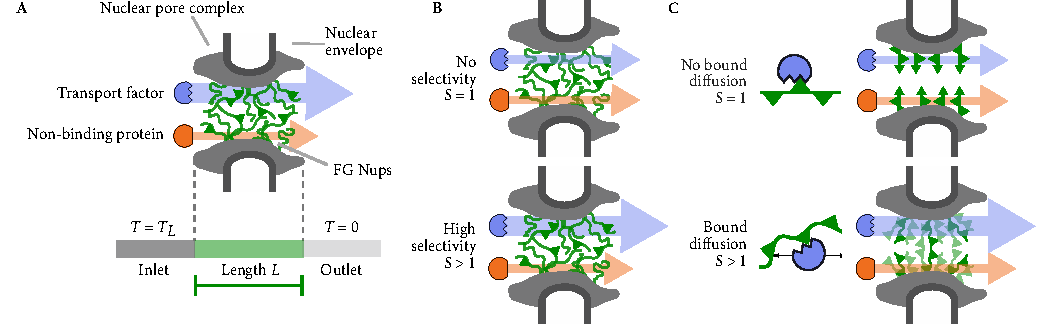
\includegraphics[width=17.8cm]{figs/ch02/fig1.pdf}
\caption[Schematics of the nuclear-pore complex and model.]{Schematics of the nuclear-pore complex and model. (A) The
  nuclear pore complex (gray) is filled with FG Nups (green polymers)
  that selectively passage transport factors that bind to FG Nups
  (blue) while blocking non-binding proteins (red). The central
  channel of the pore has length $L$. Protein concentration is high on
  the left (inlet) and low on the right (outlet).  (B) Selectivity
  quantifies the degree of selective transport through the pore. A
  non-selective pore with $S=1$ has the same flux for a transport
  factor as for a non-binding protein (top). A selective pore with
  $S>1$ has a larger flux for a transport factor than a non-binding
  protein (lower). (C) The bound diffusion coefficient quantifies the
  mobility of a bound transport factor.  A transport factor may be
  immobile (top) or mobile (lower) when bound. }
\label{fig:cartoon}
\end{figure}

Many transport factors require active release from the pore and their cargo \cite{lowe15, mincer11, gorlich96, gilchrist02}.  To avoid the complications of facilitated release, we focused on the diffusion of Nuclear Transport Factor 2 (NTF2) through the selective barrier.  NTF2 does not require active release from the pore, and, while it is at the cusp of the passive  diffusion limit at 30 kDa, its flux through the pore is approximately 30 times higher than that of a similarly-sized non-binding protein \cite{mincer11, zilman07}.  The small size of NTF2 is also a benefit in that it is significantly smaller ($\sim 5$ nm) than the depth of the nuclear pore ($\sim 100$ nm), meaning that our approximation of the pore as a bulk material is appropriate.

Our model also assumes that the rate-limiting step of nuclear transport is motion within the pore, not entry or exit.  In single-molecule measurements, most of the transport time is spent in a random walk within the central channel \cite{yang04, tu13}.

%%%%% bare-bones description of model, not sure if I should try to alter
We consider a channel of length $L$ filled homogeneously with Nups
that separates two reservoirs \figref[A]{fig:cartoon}.  A concentration diference is imposed between the two reservoirs in order to drive flux.  Within the
channel are free transport factor (concentration $T$), free FG Nups
($N$), and bound TF-FG complex ($C$), with total Nup concentration
$N_t= N+C$.  TF diffusion within the channel ($0<x<L$) is described by
the reaction-diffusion equations
\begin{eqnarray}
  \frac{\partial T}{\partial t} &=& -\kon T N+\koff C +D_F
       \frac{\partial^2 T}{\partial x^2},\label{eq:continuum_main} 
   \\ 
  \frac{\partial C}{\partial t} &=& \kon T N -\koff C + 
        D_B \frac{\partial^2 C}{\partial x^2} .
\label{eq:continuum_main_2} 
\end{eqnarray}
TF-FG interaction has on-rate constant $\kon$, off-rate $\koff$, and
dissociation constant $K_D =\koff/\kon$.  We include competition
between TFs for FG binding sites \cite{timney16}.  The
diffusion constants of free ($D_F$) and bound ($D_F$) TFs are
spatially constant. The fixed reservoir TF concentrations are $T_L$
(inlet, left) and 0 (outlet, right).

The flux of transport factor out of the pore is
$J = - D_F \left. \partial T/\partial x \right|_{x=L}$.
We defined a figure of merit, selectivity, to describe the enhancement in transport factor flux at steady-state over that of a non-binding protein (Fig.~\ref{fig:cartoon}B).  Selectivity is defined as
\begin{equation}
  S =  \frac{J_{\rm binding}(t \to \infty)}{J_{\rm non-binding}(t \to \infty)} .
\end{equation}

Mike Stefferson developed code that numerically integrated the full, nonlinear reaction-diffusion equations and calculated selectivity \cite{stefferson18}.

\subsection{Linear appoximation and analytic solution}
\label{sec:linear}
% I'm not sure whether I should put this in, because Loren was really the one who developed it.
Experimental evidence suggests that the flux of transport factors within the pore is linearly related to their concentration \cite{timney06, schmidt15}.  This would imply that few of the Nup binding motifs are occupied, so that $C \ll N$.  In this case, the concentration $N$ of un-bound Nups is approximately equal to the total Nup concentration $N_t$, a constant.  Letting $N \approx N_t$ linearizes the reaction-diffusion equations Eqns.~\ref{eq:continuum_main_2}, at which point they can be solved analytically.  The solution was developed by Loren Hough and is presented here.  The full nonlinear numerical model was used in all other sections unless noted otherwise.

% I wrote up the math here for the paper.
The analytical solution for flux can be directly derived in the linear
case.  For ease of calculation, we reverse the concentration gradient
used in the nonlinear model, so that $T(0) = 0$ and $T(L) = T_L$, allowing
us to calculate flux at $x=0$.  The reaction-diffusion equations
(\ref{eq:continuum_main}, \ref{eq:continuum_main_2}) at steady state
in the linear limit $N \approx N_t$ are
\begin{eqnarray}
0 &=& -\kon N_t T +\koff C +D_F\frac{\partial^2 T}{\partial x^2},  \\ 
0 &=& \kon N_tT -\koff C + D_B \frac{\partial^2 C}{\partial x^2} .
\label{eq:continuum_linear} 
\end{eqnarray}
The change of variables $C = C_x + N_t K_A T$ ($K_A =  \kon / \koff  = 1/K_D $ ) yields
\begin{eqnarray}
  0 &=& \koff C_x +D_F\frac{\partial^2 T}{\partial x^2}   \\ 
  0 &=& -\koff C_x  + D_B \frac{\partial^2 C_x}{\partial x^2} + N_t
        K_A  D_B \frac{\partial^2 T}{\partial x^2}.
\label{eq:continuum_change_variables} 
\end{eqnarray}
Substituting $C_x(x) = -\frac{D_F}{\koff}\partial^2T/\partial x^2$
makes equation (\ref{eq:continuum_change_variables}) a fourth-order
ODE
\begin{equation}
  \lambda^2 \frac{\partial^2 T}{\partial x^2} =  \frac{\partial^4
    T}{\partial x^4}, 
\label{continuum} 
\end{equation} 
where $\lambda^2 = \koff(D_F+ N_t K_A D_B)/(D_FD_B)$.  Solutions to
this equation have the form
$T(x) = b + m x + f e^{\lambda x} + g e^{-\lambda x}$, where
$b,\ m,\ f$ and $g$ are constants fixed by four boundary conditions:
free TF concentration is fixed at the edges of the pore, with
$T(0) = 0 $, $T(L)=T_L$. No flux of bound TF into or out of the pore
occurs, giving $\partial C/\partial x |_{x=0} =0$,
$\partial C/\partial x|_{x=L} = 0$.  The constants of integration are
\begin{eqnarray}
b&=& - (f+g),\\
m & =& \frac{T_L\lambda \left( \zeta -(D_F/\koff) {\lambda}^2\right) \left(e^{L \lambda} + 1\right)}{2  \zeta - 2  \zeta e^{L \lambda} + L  \zeta \lambda -(D_F/\koff) L {\lambda}^3 -(D_F/\koff) L {\lambda}^3 e^{L \lambda} + L  \zeta \lambda e^{L \lambda}},\\
f &=& -\frac{ \zeta m}{\lambda \left( \zeta -(D_F/\koff) {\lambda}^2\right) \left(e^{L \lambda} + 1\right)},\\
g &=& \frac{ \zeta m + f  \zeta \lambda- (D_F/\koff) f {\lambda}^3 }{ \zeta \lambda -(D_F/\koff) {\lambda}^3}.
\end{eqnarray}
where $\zeta = N_t/K_D$. This leads to a concentration profile of bound TFs 
\begin{equation}
C(x) = \zeta \left(b + m x + f e^{\lambda x} + g e^{- \lambda
    x}\right) - (D_F{\lambda}^2/\koff)   \left(ge^{- \lambda x} + f
  e^{ \lambda x}\right). 
\end{equation}

To determine the selectivity, we calculate the steady-state flux out
of the pore\\ $ J =- D_F \partial T/\partial x|_{x=0}$, giving
\begin{eqnarray}
J& =&-D_F( m + \lambda f - \lambda g) \\
J&=& \frac{{T_L (D_F^2/\koff) { \lambda}^3 \left(e^{L  \lambda}
     + 1\right)}}{2 \zeta - 2 \zeta e^{L  \lambda} + L \zeta
     \lambda - (D_F/\koff) L  \lambda^3 - (D_F/\koff) L  \lambda^3
     e^{L  \lambda} + L \zeta  \lambda e^{L  \lambda}} 
\end{eqnarray}
For a non-binding particle, $C(x) = 0$, $T = T_L x / L$, and
\begin{equation}
  J_n =-\frac{D_F T_L}{L}. 
\end{equation}
The selectivity $J/J_n$ is then independent of $T_L$ in
the linear approximation.

\subsection{Effect of bound-state diffusion constant}

\begin{figure*}[t!]
\centering
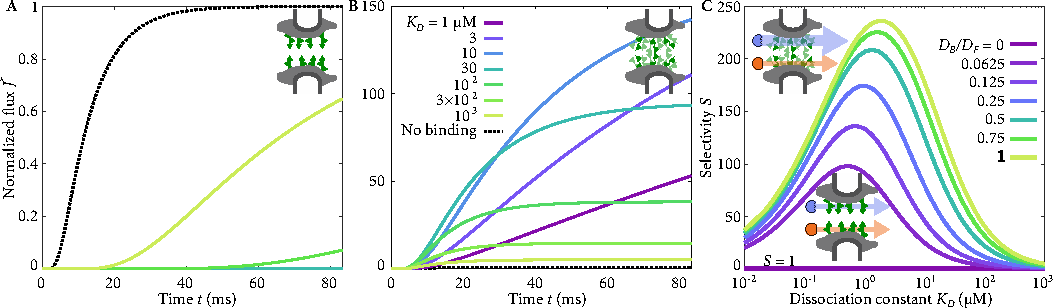
\includegraphics[width=\textwidth]{figs/ch02/fig2.pdf}
\caption[Flux and selectivity as a function of bound mobility.]{Flux through the pore and selectivity for TFs with varying
  bound mobility. (A) Flux as a function of time when TFs are immobile
  while bound, with varying binding affinity as in (B).  (B) Flux as a function
  of time when TFs are mobile while bound with $D_B = D_F$, with
  varying binding affinity.  (C) Selectivity as a function of
  dissociation constant with varying bound diffusion coefficient. }
\label{fig:transient}
\end{figure*}

When the selectivity is calculated for the full nonlinear equations, bound-state mobility is immediately obvious as the key parameter.  We were unable to create a selective material if the bound diffusion constant $D_B$ was set to zero, i.e. if the Nup-transport factor complex was immobile while bound.  In those cases, the steady-state flux of transport factor and inert protein was identical regardless of the values chosen for $\kon$ or $\koff$ giving a selectivity of $S = 1$.  The transient flux ratio did depend on binding kinetics, as shown in Figure~\ref{fig:transient}A and B.  As would be expected, the transient flux of transport factor out of the material was suppressed relative to that of the inert protein, as a population of the transport factor filled binding sites throughout the material.  Once binding equilibrium has been established, however, the immobile population of bound transport factors cannot contribute to the flux out of the pore, and the steady-state flux of binding and non-binding proteins is identical.

However, when bound-state mobility is allowed and $D_B > 0$, the system's selectivity can greatly increase, as shown in Figure~\ref{fig:transient}C.  The transient response is dramatically different as well.  Now transport factor flux very rapidly outpaces that of inert protein.  It should be noted that the timescale for equlibration is similar to that observed experimentally for NTF2, approximately 10 ms.

In order to create these plots, we used the FG-filled pore length $L = 100\ \nm$
\cite{frenkiel-krispin10, maimon12}.  Total FG Nup concentration was determined from an estimate of the number of TF binding sites (800), and the volume of a cylinder of diameter $60\ \nm$ and length $L$.  Finally, an estimate of the free diffusion constant of NTF2 moving within the nuclear pore is needed.  This value has not been directly measured, but it was estimated at $D_F = 0.12 \ \mu\tx{m}^2$/s using a similar value for a non-binding protein \cite{ribbeck01}.  As would be expected, this diffusion constant is smaller than that of a karyopherin in the nucleus, which has been estimated at $D_F =1 \ \mu\tx{m}^2$/s \cite{cardarelli10}.  In order to estimate the concentration gradient between nucleus and cytoplasm, we need to know the concentration of transport factor just inside the cytoplasmic side of the nuclear pore.  There will be an energy barrier to any protein entering the pore because of the entropic penalty of the Nups.  We estimate this barrier is approximately $1.5\ k_B T$ for an NTF2 sized molecule \cite{timney16}.  We estimate the cytoplasmic concentration of NTF2 is 5 $\mu$M.  Then $T_L= 5 \times e^{-1.5} \mu \tx{M} = 1 \tx{\ \mu M}$.  

Experimental evidence suggests that the on-rate constant of Nup-transport factor binding is diffusion-limited, with $\kon = 10^{-3}\mu \tx{M}^{-1} \, \mu \tx{s}^{-1}$ \cite{milles15, hough15}.  The off-rate constant is given by $\koff ~=~\kon K_D$.  Measured values of the dissociation constant $K_D$ span several orders of magnitude, between approximately between 10 nM and 10 $\mu$M \cite{pyhtila03, gilchrist02, tetenbaum-novatt12-1,
  milles15, timney16, vovk16}; therefore the off-rate constant is not well-determined.  Figure~\ref{fig:tethers}B and C show the bound diffusion coefficient and selectivity for a range of $K_D$ values spanning those measured experimentally, with a fixed, diffusion-limited on-rate.  Throughout this work, we consider a wide range of dissociation constants.

This model provides a straightforward method of predicting the selectivity of various other hydrogel nuclear pore mimics \cite{frey09,ader10,frey07,kim15}.  A table of predicted selectivity is provided in Appendix~\ref{appx:npc-mimics}.

Allowing the bound diffusion constant to approach the free diffusion constant, using the above parameters, selectivity can approach the values seen in experimental measurements (Table \ref{table:NTF2-flux}).  The interplay between binding kinetics and diffusion leads to an optimal dissociation constant near 1~$\mu$M for maximum selectivity (\figref[C]{fig:transient}). Selectivity decreases for high $K_D$ because binding is too weak to
significantly increase TF concentration in the pore.  For low $K_D$, tight binding causes the concentration of bound complexes to become approximately constant across the pore, eliminating the concentration gradient needed to provide flux across the pore.

%In systems such as airway mucus,
%immobilization may increase the time available for degradation or
%active clearance, consistent with the observation that binding tends
%to inhibit selective transport in those systems \cite{schneider17,
%  huang17, mastorakos15}.  This effect is related to the binding-site
%barrier seen in antibody delivery to tumors \cite{juweid92}, and
%observations that non-binding nanoparticles are often more effective
%in drug delivery to tumors than binding particles \cite{witten17}.

%Our model is related to the classic problem of molecular transport
%through an oil membrane separating two aqueous reservoirs
%\cite{schafer13}.  The relative concentration of a species just inside
%the oil barrier to the concentration in water is called the partition
%coefficient.  The steady-state flux through the membrane is directly
%proportional to the partition coefficient (Supporting Information,
%section \ref{sec:partition}, fig.~\ref{fig:oil-membrane}).  By
%analogy, one might expect the TF-FG binding affinity to determine the
%flux across the pore. However, binding is different from partitioning.
%In systems where the increase in intra-pore concentration arises from
%binding, the effective diffusion coefficient is typically inversely
%proportional to the partition coefficient, making the flux independent
%of binding affinity \cite{bickel02}.  This result led us to consider
%whether TFs may be mobile while bound to FG Nups.

\begin{table}[b!]
  \caption[Comparison between flux measurements and model predictions.]{Comparison between experimental results for NTF2 and GFP
    (a similarly-sized non-binding protein) and model
    predictions. Flux measured in units of molecules per pore per
    second.}
    \label{table:NTF2-flux}
    \begin{tabular}{p{2.1cm}p{1.2cm}p{1.7cm}p{0.9cm}p{1.6cm}p{0.8cm}}
      Method & Cell type & Species & Flux & Selectivity & Notes\\
      \hline
      OSTR & \textit{Xenopus} & \makecell[cl]{NTF2\\GFP} & \makecell[cl]{91--123\\3.3--3.8} & 24--37 
                         &\cite{siebrasse02}
      \\
      OSTR & \textit{Xenopus} & \makecell[cl]{NTF2\\GFP} & \makecell[cl]{47.3\\1.1} & 43 &  \cite{kiskin03}\\
      \makecell[cl]{Permeabilized \\ cells}  & HeLa &
                                                    \makecell[cl]{NTF2\\GFP} & \makecell[cl]{250\\2} & 125 & \cite{ribbeck01}\\
      Model & -- & \makecell[cl]{Binding\\Non-binding} & \makecell[cl]{2--480\\2} & 1--240 & \makecell[cl]{This\\work}\\
    \end{tabular}
\end{table}

\subsection{Bound diffusion in the linear model}

In the linear approximation described in Sec.~\ref{sec:linear}, bound diffusion plays a similar role as in the full nonlinear model.  By definition, the Nup binding sites don't saturate in the linear model.  This leads to a plateau in the selectivity at tighter binding, rather than a peak (Fig~\ref{fig:linear-selectivity}).  However, the linear model becomes non-physical for $K_D < N_t$, denoted by the dotted line in Fig.~\ref{fig:linear-selectivity}C.

The role of individual parameters can be more easily investigated using the linear approximation.  Figure~\ref{fig:parameter-variations} illustrates the effect on selectivity of varying the on-rate constant, total FG Nup concentration, free diffusion constant, and pore length.  Figure~\ref{fig:parameter-variations-abs-flux} does the same for the absolute flux of transport factor through the pore.  These results show that increasing the on-rate constant or the total Nup concentration results in both higher selectivity and transport factor flux, a conclusion which is supported by the fact that these values are maximized within the nuclear pore \cite{milles15, hough15}.  However, there is a trade-off between selectivity and flux for the pore length and free diffusion constant.  Increasing pore length or decreasing free diffusion constant make the pore more selective but lower the absolute flux of transport factor.

\begin{figure}
\centering
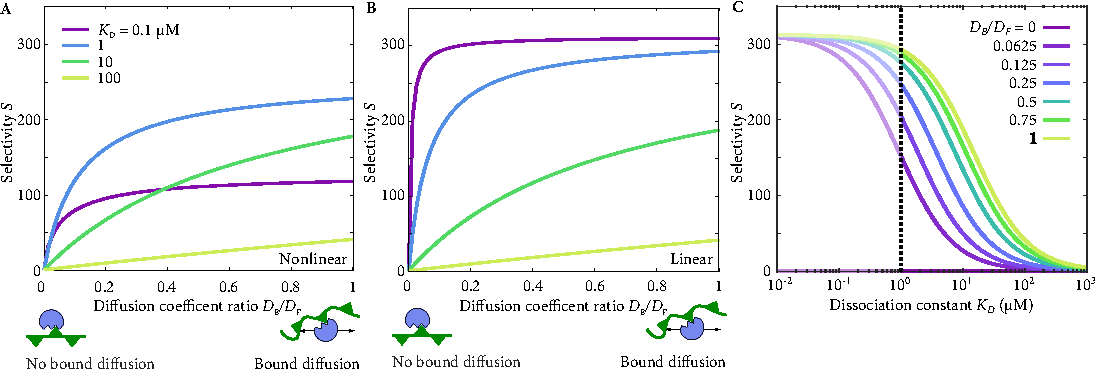
\includegraphics[width=\linewidth]{figs/ch02/linear-selectivity.pdf}
\caption[Selectivity in the linear approximation.]{(a, b) Selectivity as a function of diffusion coefficient
  ratio, with varying dissociation constant, in the full nonlinear
  model (a) or in the linear approximation (b).  (c) Selectivity as a
  function of dissociation constant, with varying diffusion
  coefficient ratio, in the linear approximation.  The region to the
  left of the dotted line is non-physical; the full nonlinear solution
  should be used.}
\label{fig:linear-selectivity}
\end{figure}

\begin{figure}
\centering
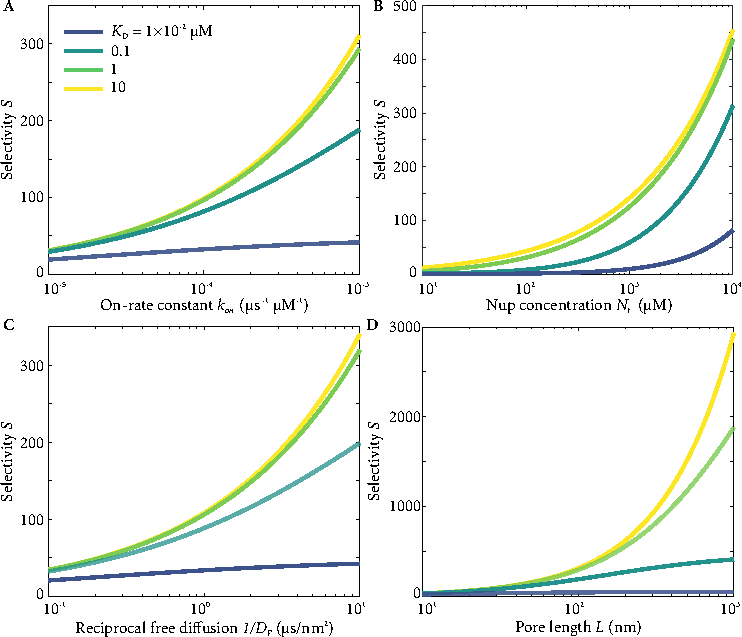
\includegraphics[width=0.7\linewidth]{figs/ch02/parameter-variations.pdf}
\caption[Dependence of selectivity on model parameters.]{Dependence of selectivity on variation of individual
  parameters: (a) on-rate constant, (b) total FG Nup concentration, (c) inverse of the free diffusion coefficient, and (d) pore
  length, with varying dissociation constant. All values calculated using the linear solution to the binding-diffusion equations.  Bound diffusion coefficient $D_B = 0.1D_F$. Other parameters fixed at values from the NPC parameters section.}
\label{fig:parameter-variations}
\end{figure}

\begin{figure}
\centering
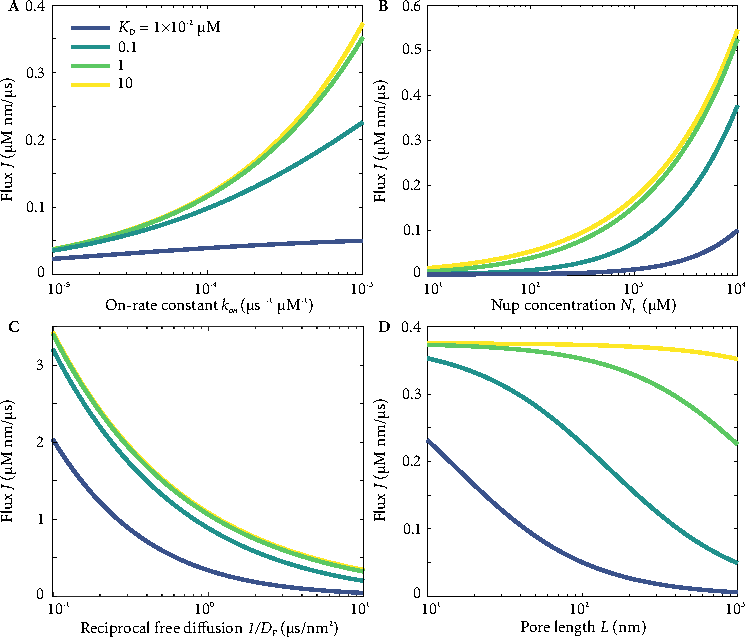
\includegraphics[width=0.7\linewidth]{figs/ch02/parameter-variations-abs-flux.pdf}
\caption[Dependence of absolute flux on model parameters.]{Dependence of flux on variation of individual parameters: (a)
  on-rate constant, (b) total FT Nup concentration $N_t$, (c) inverse
  of the free diffusion coefficient, and (d) pore length, with varying
  dissociation constant. All values calculated using the linear solution to the binding-diffusion equations. Bound diffusion coefficient $D_B = 0.1D_F$. Other parameters fixed at values from the NPC parameters section.}
\label{fig:parameter-variations-abs-flux}
\end{figure}


\section{Mechanisms of  bound transport factor mobility}

The importance of bound diffusion to selectivity in our model raises the question of how transport factor- Nup complexes might diffuse within the pore.  The following sections describe two possible mechanisms of bound-state diffusion within the nuclear pore: tethered diffusion and inter-chain hopping due to binding multivalency.  Both mechanisms are appealing because they rely only on well-established properties of Nups and transport factors.  Our results suggest that each mechanism could contribute significant selectivity.

\section{Bound mobility through tethered diffusion}
%I wrote the math for this section of the paper
One possible mechanism of bound-state diffusion within the nuclear pore is tethered diffusion.  FG Nups, as disordered proteins, are flexible and highly dynamic \cite{lim07, milles14, hough15,patel07}. It is not clear whether they form polymer brushes or crosslinked hydrogels within the nuclear pore, but in either case tethered diffusion remains a viable mechanism of bound diffusion.  In the case of a polymer brush, one end of an FG Nup is anchored to the NPC scaffold, but the other end is free, affording mobility to a bound transport factor.  If FG Nups are crosslinked, the effective length of the flexible tether will be shorter, but the same principle of tethered diffusion will apply.

Flexible polymers behave as entropic springs \cite{howard01} if they are not highly stretched. Therefore, a bound TF diffuses while attached to a spring-like tether, which can be represented as diffusion in a harmonic potential well \figref[A]{fig:tethers}.  The width of the harmonic well is related to the length of the flexible domain.  The effective length is the full FG Nup length if the FG Nups are not crosslinked, while the effective length is reduced if they are crosslinked or entangled\cite{ribbeck01}.  

In order to calculate the bound diffusion coefficient of the TFs, an averaging procedure is followed.  The diffusion is assumed to be Fickian, which is a reasonably good though not perfect assumption. (See discussion in Sec.~\ref{sec:fickian}.)  In the Fickian diffusion case, the diffusion coefficient is proportional to a mean-squared displacement (MSD) divided by time.  We calculate the mean binding lifetime $\tau$ and the MSD corresponding to this ``typical'' binding event and divide them.

To begin, note that the duration of a binding event follows the exponential distribution 
\begin{equation}
\rho (t) = \exp(-t/\tau)/\tau\,,
\end{equation}
where $\tau = 1/\koff$ is the mean binding lifetime.

Next, the positional probability density of a bound TF is 
\begin{eqnarray}
P(x,t) &=& e^{-\frac{x^2}{2 \alpha(t)}}/\sqrt{2\pi \alpha(t)}\,,\\
\alpha(t) &=& (1-e^{-2kD_F\beta t})/(k\beta)
\end{eqnarray}
 where $k$ is the spring constant of FG Nup tethering and $1/\beta = k_BT$ is the thermal energy \cite{doi88}.  The center of the well is set at $x=0$.

The mean-squared displacement (MSD) of the TF as a function of time is calculated, as any expected value, with the integral
\begin{equation}
\ev{x^2(t)} = \int_{-\infty}^{\infty} P(x,t) x^2 dx = \alpha(t)\,.
\end{equation}

Finally, the typical TF MSD during a binding event can be determined by evaluating
\begin{equation}\label{eq:sho}
  \overline{\ev{x^2}} = \int_0^{\infty} \rho(t') \ev{x^2(t')} dt' = \frac{2D_F L_c
    \ell_p}{L_c \ell_p \koff+ 3D_F}\,. 
\end{equation} % Mike realized this was actually a pretty easy integral - should I credit him here?
Here we assume that the spring constant is that of a worm-like chain polymer $k = 3/(2\beta L_c \ell_p)$, where $L_c$ is the contour length and $\ell_p$ the persistence length \cite{howard01}.

Combining these results, the one-dimensional bound diffusion coefficient is
\begin{equation}\label{eq:dbound}
  D_B \approx \frac{\overline{\ev{x^2}}}{2\tau} = \frac{D_F L_c \ell_p
    k_\un{off}}{L_c \ell_p k_\un{off} + 3D_F} =
  \frac{D_F}{1+3\frac{D_F}{D_{P}}}.  
\end{equation}
Here $D_P = L_c \ell_p k_\un{off}$ controls the bound-state diffusion coefficient: higher $D_P$ corresponds to a lower constraint of the TF by the tether and greater bound mobility. Bound mobility increases with increasing chain length and persistence length, or decreasing binding lifetime. When $D_P$ is large ($D_F/D_P\ll1$), $D_B$ approaches $D_F$, since the long chains barely affect TF motion during the short binding event. For small $D_P$ ($D_F/D_P\gg1$), TF motion is inhibited by a short tether, giving $D_B\approx D_P/3\ll D_F$.  

\begin{figure}
\centering
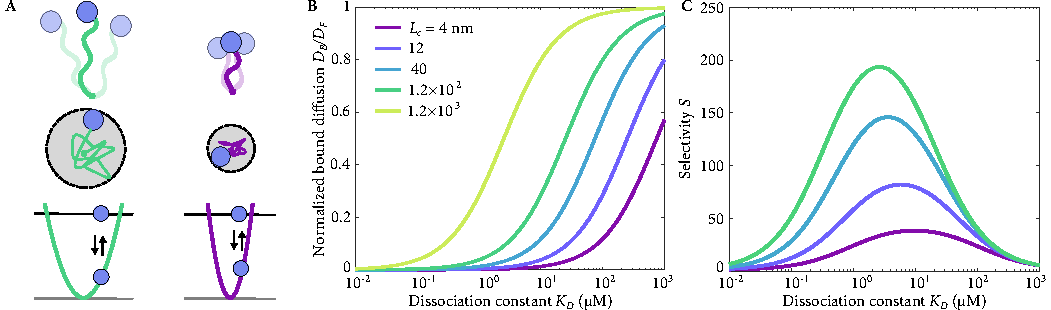
\includegraphics[width=\textwidth]{figs/ch02/fig3.pdf}
\caption[Selectivity from tethered diffusion.]{(A) Schematic of the flexible tether model of bound-state
  diffusion. FG Nups are treated as entropic springs that constrain
  the motion of TFs more (top and center left, longer FG Nup) or less
  (top and center right, shorter Nup), which corresponds to changing
  width of the harmonic potential well (lower).  (B) Ratio of bound to
  free diffusion coefficient as a function of dissociation constant,
  with varying polymer length in the tethered-diffusion model.  (C)
  Selectivity as a function of $K_D$, with varying polymer length in
  the tethered-diffusion model.  Selectivity calculated by Mike Stefferson.}
\label{fig:tethers}
\end{figure}

Physiological values can be estimated for all of the relevant parameters.  Disordered proteins are relatively flexible, with persistence lengths around $\ell_p \approx 1$ nm \cite{receveur-brechot12}.  The contour lengths of the disordered regions of FG Nups are in the range $L_c\approx$ 100--280 nm (250--700 amino acids long \cite{patel07} with a contour length per amino acid $\approx 0.4$ nm).

\begin{SCfigure}
\centering
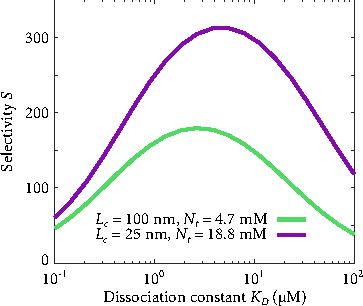
\includegraphics[width=0.4\textwidth]{figs/ch02/chain-comparison.pdf}
\caption[Nup contour length and concentration comparison.]{Selectivity as a function of dissociation
  constant in the tethered diffusion model, varying Nup contour length $L_c$ and total Nup concentration $N_t$.  The product $L_cN_t$ is held constant.\\}
\label{fig:chainComparison}
\end{SCfigure}

Using these parameters, along with those described in earlier sections, Mike Stefferson calculated the selectivity due to tethered diffusion for several tether lengths (Fig.~\ref{fig:tethers}C).  Selectivity was also calculated for two values of the total Nup concentration $N_t$, mimicking the possible effect of Nup crosslinking within the pore (Fig~\ref{fig:chainComparison}.  The produce of contour length and Nup concentration $L_cN_t$ was held constant, and selectivity calculated for a long Nup length of 100 nm as well as a shorter length of 25 nm, reflecting the possibility of crosslinking.  Corresponding total Nup concentrations of 4.7 and 18.8 nm, respectively, were determined from an estimate of the number of TF binding sites ($800$), and the volume of a cylinder of diameter $60\ \nm$ and length $L = 100$ nm. 

 Using these realistic parameters, selectivity can reach 200-300, a large flux enhancement for TFs over nonbinding proteins.

\section{Bound mobility through inter-chain hopping}
\label{sec:hopping}

Another possible mechanism of bound-state diffusion is inter-chain hopping enabled by multivalent binding interactions.  All known transport factors have at least two hydrophobic binding pockets which bind to FG motifs, and some have many more \cite{wagner15}.  FG Nups in turn each possess many FG motifs, leading to a highly multivalent binding interaction.  This feature allows a transport factor to bind to multiple Nups at once, moving between them with a hand-over-hand or sliding motion without ever fully unbinding \cite{raveh16, tetenbaum-novatt12}.  While binding to multiple FG motifs on the same Nup will not lead to bound diffusion, inter-chain hopping will cause the origin site of tethered transport factor diffusion to change over time.  In order to understand the effect of hopping on the overall bound diffusion constant, we model a TF that undergoes tethered diffusion when bound to an FG Nup and hops between neighboring, randomly distributed tethers \figref{fig:hopping}.

\begin{figure*}
\centering
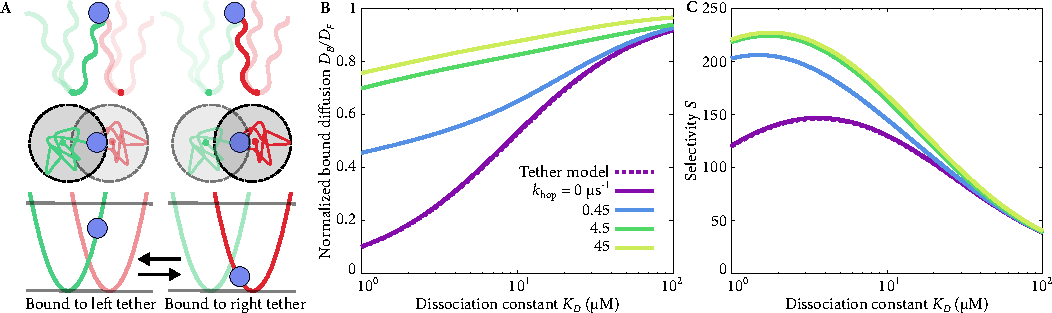
\includegraphics[width = \textwidth]{figs/ch02/fig4.pdf}
\caption[Selectivity from inter-chain hopping.]{(A) Schematic of the inter-chain hopping model of bound-state diffusion. FG Nups are treated as entropic springs that constrain the motion of TFs, and inter-chain hopping allows a TF to move from one FG Nup (top and center left, green Nup) to another (top and center right, red Nup) without unbinding, which corresponds to switching from one harmonic potential well to another (lower). (B) Ratio of bound to free diffusion coefficient as a function of dissociation constant, with varying hopping rate in the inter-chain hopping model.  (C) Selectivity as a function of $K_D$ with varying hopping rate. FG Nup contour length $L_c = 40$ nm in (B, C). }
\label{fig:hopping}
\end{figure*}

In our simulation of TF motion with hopping between FG Nups while bound, we represented each FG Nup as an entropic spring (i.e. as a harmonic potential well).  Well positions were randomly chosen from a uniform distribution, with the exception that we always placed one well at the starting position of the TF.  The particle (the TF) started the simulation bound to this FG Nup, and remained bound throughout the simulation.  While bound to one FG Nup, the TF diffused within the harmonic well representing that FG Nup. We recorded the position and mean-squared displacement of the TF from its starting location, which we then used to determine a bound diffusion coefficient, as described in more detail below.  The TF could hop between tethers by changing which well it moved in.

The source code of the hopping simulation is available at \url{https://github.com/LauraMaguire/hoppingSim}.

% I wrote all of the sections below, describing the hopping simulation, for the paper.
\subsection{Diffusion in a potential well}

The TF moved in the harmonic potential of the FG Nup according to Brownian dynamics. At each timestep, the TF position was updated using a force-dependent diffusive step \cite{blackwell17}.
\begin{equation}
  x(t+\delta t) = x(t) + \frac{F}{\Gamma} \delta t + \delta x\,,
\end{equation} 
where $F$ is the force acting on the particle, $\Gamma$ is the drag coefficient, $\delta t$ is the timestep, and $\delta x$ is a random Brownian step drawn from a Gaussian distribution with variance $\sigma^2 = 2 D \delta t$. The drag coefficient of a spherical particle at low Reynolds number is given by Stokes' Law as $\Gamma = 6 \pi \eta r$, where $\eta$ is the fluid's viscosity and $r$ is the sphere's radius.  This result can be combined with the Einstein relation $D = k_B T / (6\pi \eta r)$ to give
\begin{equation}
\Gamma= \frac{k_B T}{D}\,.
\end{equation}
 
The force $F = -k\Delta x$, where $k$ is the spring constant of the FG Nup and $\Delta x$ is the displacement of the particle from the Nup attachment point.  We model the FG Nup as a worm-like-chain at small extension, so that $k = 3 k_B T/(2\ell_pL_c)$, where $\ell_p$ is the tether persistence length and $L_c$ is the contour length.  Then 
\begin{equation}
  x(t+\delta t) = x(t) - \frac{3 D \Delta x \delta t}{2\ell_p L_c }+
  \delta x = x(t) - D K \Delta x \delta t+ \delta x\,,
\end{equation}
where $K$ is the normalized spring constant $K = k/k_B T = 3/(2 \ell_p L_c)$.

\subsection{Hopping probability}

We designed the hopping probability $\Phop$ in order to satisfy the principle of detailed balance.  During every iteration of the simulation, we picked an FG Nup at random from a list of the $M$  Nups near enough to have a reasonable probability of hopping. TF hopping to the new FG Nup was attempted with success probability
\begin{equation}
\Phop = r_\tx{hop} M \delta t e^{-\Delta G /2}.
\end{equation}
Here the base hopping rate $r_\tx{hop}$ is a dimensionless input parameter, and the change in free energy (in units of $k_BT$) between the current Nup and the proposed new Nup is
\begin{equation}
  \Delta G = \frac{1}{2} K (x-x_\tx{new})^2 - \frac{1}{2} K (x -
  x_\tx{cur})^2,
\end{equation}
where $K$ is the normalized spring constant, $x$ is the particle's current position, $x_\tx{cur}$ is the anchor location of the Nup to which the particle is currently bound, and $x_\tx{new}$ is the anchor location of the proposed new Nup. Note that when a hop succeeds, the energy landscape changes to that of the new Nup, but the TF's position does not change during the hop.  There is no upper bound on $\Phop$, but we adjusted the timestep to ensure that $\Phop$ was greater than
unity no more than 0.5\% of the time that a hop was attempted.

\subsection{Mean-squared displacement and diffusion coefficient calculation}
We ran each simulation for $10^7$ time steps with $\delta t = 0.01$ $\mu$s, and recorded the particle's position every 100 time steps.  We calculated the mean-squared displacement $\ev{x^2}$ (MSD) of the TF and averaged it over 100 runs \figref[A]{fig:integrand}.  We then computed
\begin{equation}
\rho_\tx{MSD} (t)= \ev{x^2(t)} \rho(\koff,t) = \koff \ev{x^2(t)}
e^{-\koff t}, 
\end{equation}
as shown in fig.~\ref{fig:integrand}B, and numerically integrated the distribution in time. We determined the bound diffusion coefficient from the typical MSD-per-binding-event $\overline{\ev{x^2}}$ using
\begin{equation}
D_B = \frac{\koff \overline{\ev{x^2}}}{2}. 
\end{equation}   
Here, the factor of $1/2$ is appropriate because we consider a one-dimensional random walk.

\begin{figure}[h!]
\centering
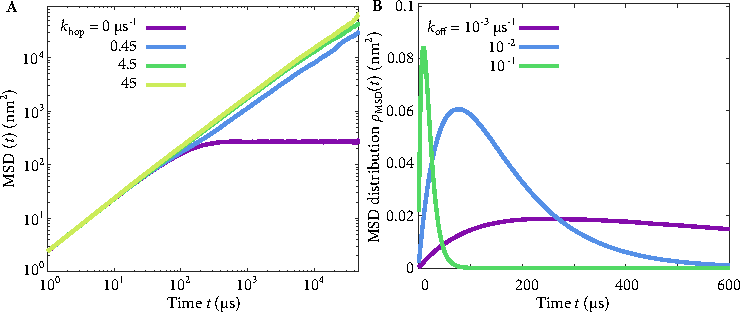
\includegraphics[width=0.7\linewidth]{figs/ch02/integrand-example-plots.pdf}
\caption[Mean-squared displacement in the hopping simulation.]{(A) Examples of mean-squared displacement (MSD) of a simulated TF in the inter-chain hopping model, with varying hopping rate.  (B) Examples of MSD distributions $\rho_\tx{MSD} (t)$ used in estimating the diffusion coefficient, with varying unbinding rate. Tethers have 40 nm contour length; other parameters are as discussed in the text.}
\label{fig:integrand}
\end{figure}

\subsection{Bound diffusion and selectivity from hopping simulation}

Upon calculating the bound diffusion constant using the hopping simulation described above, it was clear that inter-chain hopping could lead to relatively large bound diffusion constant, with a corresponding increase in selectivity (Figs.~\ref{fig:hopping}, \ref{fig:hop-results}).  In the limit of a hopping rate of zero, the tethered-diffusion-only result is recovered, as anticipated.  Hopping most enhances selectivity when the Nup length or dissociation constant are small.  This is the regime where tethered diffusion is limited, corresponding to crosslinked Nups within the nuclear pore.  If the pore is highly crosslinked, binding multivalency may be essential to selectivity.

\begin{figure}
\centering
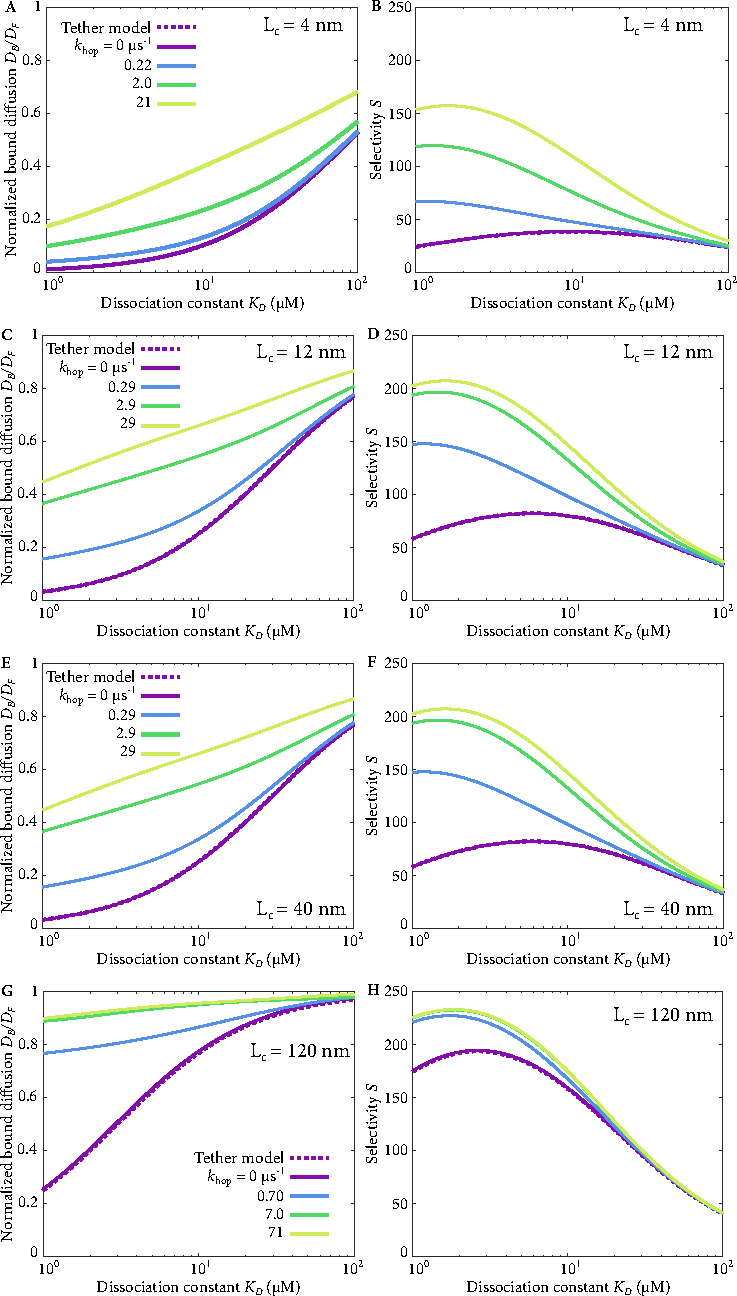
\includegraphics[width=0.7\linewidth]{figs/ch02/hopping_lc4-fig.pdf}
\caption[Effect of Nup contour length and hopping rate on selectivity.]{Bound diffusion and selectivity as a function of dissociation
  constant, with varying hopping rate for FG Nups with (A,B) $L_c = 4$ nm; (C,D) $L_c = 12$ nm; (E,F) $L_c = 40$ nm; (G,H) $L_c = 120$ nm.}
\label{fig:hop-results}
\end{figure}
%\begin{figure}[h]
%\centering
%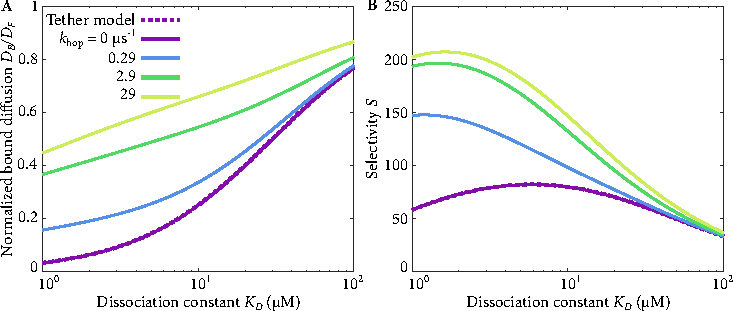
\includegraphics[width=0.7\linewidth]{figs/ch02/hopping_lc12-fig.pdf}
%\caption{Bound diffusion and selectivity as a function of dissociation
%  constant, with varying hopping rate for FG Nups with $L_c = 12$ nm.}
%\label{fig:partitioningC}
%\end{figure}
%\begin{figure}[h]
%\centering
%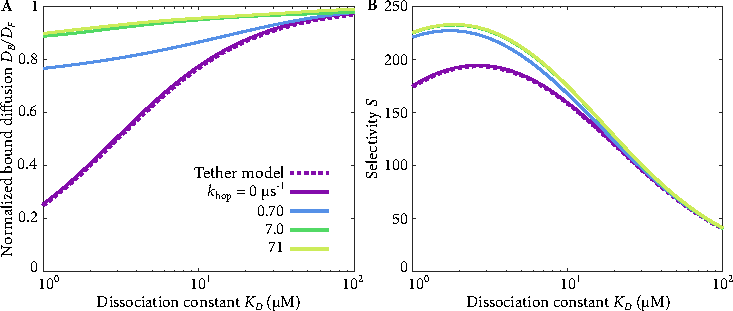
\includegraphics[width=0.7\linewidth]{figs/ch02/hopping_lc120-fig.pdf}
%\caption{Bound diffusion and selectivity as a function of dissociation
%  constant, with varying hopping rate for FG Nups with $L_c = 120$ nm.}
%\label{fig:partitioningD}
%\end{figure}

\section{Fickian and anomalous diffusion}
\label{sec:fickian}
A particle whose mean-squared displacement is proportional to time ($\langle x^2(t) \rangle \propto t$) is said to be undergoing normal or Fickian diffusion.  This is generally the case for a freely-diffusion particle with no driving forces acting upon it.  Anomalous diffusion is the more general case where $\langle x^2(t)\rangle \propto t^\alpha$.  When $\alpha > 1$, the motion is superdiffusive; $\alpha < 1$ is the subdiffusive regime, typically caused by confined diffusion or binding.

Throughout this analysis, we have assumed that all proteins are experiencing Fickian diffusion.  For inert, nonbinding proteins, this is true provided we neglect any steric confinement from the presence of the FG Nups.  Additionally, transport factors should show normal diffusion over timescales much longer than their binding lifetime.  However, binding interactions will result in slightly subdiffusive motion on shorter timescales.

In order to quantify the extent of anomalous diffusion, we ran a modified version of the hopping simulation described in Sec.~\ref{sec:hopping} in which the transport factor was not solely limited to hopping but also able to entirely unbind from and rebind to Nups with rates $\koff$ and $\kon$ respectively.  

 In order to quantify the extent of anomalous diffusion, we ran the same simulations described above but allowed total unbinding and rebinding to occur, not just hopping while bound.  The resulting MSD $\langle x^2(t) \rangle$ can then be used to investigate anomalous diffusion.  Figure~\ref{fig:anomalous-diffusion} is a log-log plot of $\langle x^2(t) \rangle/t$ vs time $t$, generated using a script created by Mike Stefferson \cite{stefferson18}.  In such a plot, a horizontal asymptote indicates Fickian diffusion, while a non-zero slope $m$ indicates anomalous diffusion with $m = \alpha -1$.

Figure~\ref{fig:anomalous-diffusion} shows several hopping rates.  When the transport factor is not able to hop between Nups, diffusion remains anomalous until well past the binding lifetime $1/\koff$ (not shown).  Larger hopping rates cause diffusion to become Fickian over shorter timescales.  The hopping lifetime $1/k_\mathrm{hop}$ is shown for each nonzero hopping rate, as well as the binding lifetime ($\koff = 10^{-4}$ $\mu$s in all cases).  The time to explore the potential well caused by binding to Nups is also shown.  The vertical line marks the experimentally-measured time for NTF2 to pass through the nuclear pore, $t_\mathrm{NTF2} = 10$ ms.

The anomalous diffusion plot indicates that the diffusion of transport factors is not entirely Fickian, but that shorter binding lifetimes and higher hopping rates lead to less anomalous diffusion.

\begin{SCfigure}
\centering
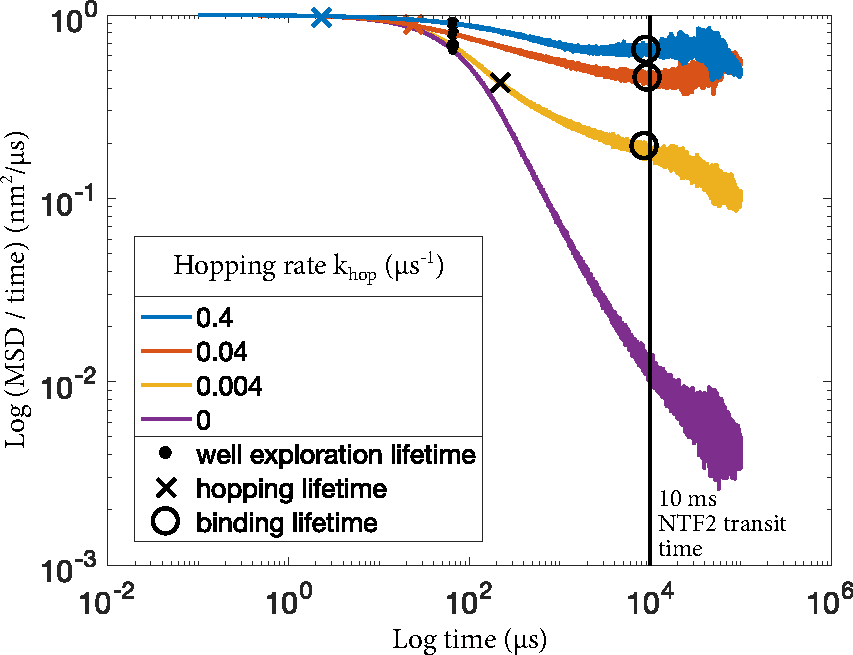
\includegraphics[width=0.5\linewidth]{figs/ch02/171103-DvsT-with-lifetimes.pdf}
\caption[Anomalous diffusion in the hopping simulation.]{Anomalous diffusion of transport factors at several hopping rates.  The hopping, binding, and well-exploration lifetimes are also shown where applicable.  NTF2 transit time (10 ms) is indicated with a vertical line.\\}
\label{fig:anomalous-diffusion}
\end{SCfigure}

\section{Bound diffusion in other biological systems}
\label{sec:other-filters}
%A key puzzle of the NPC is how transport-factor binding allows rapid transport through the pore.  Binding typically immobilizes the bound particle, and so the increase in concentration resulting from binding does not, in general, result in increased flux. The biophysical theory
%we developed includes diffusion of TFs due to thermal fluctuations,
%binding to polymeric tethers, and the hopping of bound species between
%these tethers.  Thus we identified principles of selective transport
%resulting from binding \figref{fig:cartoon}, emphasizing that
%bound-state mobility is essential for selective transport
%\figref{fig:transient}.  Binding increases the local concentration,
%and any bound mobility increases the flux.  We characterized two
%mechanisms to obtain bound-state mobility and found that
%thermally-driven diffusion of TFs bound to flexible tethers and rapid
%binding kinetics \cite{hough15, milles15} allow TF mobility, leading
%to selectivity similar to that observed experimentally
%\figref{fig:tethers}.  In addition, tether flexibility enables
%multivalent bound particles to hop between binding regions
%\figref{fig:hopping} \cite{lowe15, schoch12}, further enhancing
%selectivity. Mobility of bound or partitioned molecules occurs in many
%biological contexts, suggesting that the mechanisms we study here may
%be broadly applicable \cite{stefferson17, braga07}.
%
%
%Our model for selective transport by tethered diffusion generalizes to
%a range of FG-FG interactions \cite{vovk16}, if we decrease the
%effective chain length $L_c$ for cohesive FG Nups.  For short chains
%the selectivity simply due to chain flexibility is modest, suggesting
%that other mechanisms, like hopping, may be important.  Our model
%suggests that transient cross-linking of FG repeats proposed to occur
%within the pore may serve to increase the viscosity and therefore the
%selectivity. Crosslinks need not be actively melted by TFs to enhance
%selectivity \figref{fig:parameter-variations}.
%  
%Our model provides a quantitative tool to evaluate selective
%transport. Materials formed \textit{in vitro} by spontaneous
%self-assembly of FG Nups \cite{frey07} or transient crosslinking by
%alpha-helical peptides \cite{kim15} show strong selective
%\textit{entry}.  Using published data, we predicted whether these gels
%also showed selective \textit{transport} (table \ref{table:Gorlich}).
%Most synthetic gels are predicted to have $S<10$, less than the
%selectivity of NTF2 in cells (table \ref{table:NTF2-flux}). The
%predicted selectivity of one hydrogel is $S\approx200$, apparently the
%most selective synthetic gel to date \cite{frey07}.
%
%
%\subsection{Overcoming the limitations of binding}
%Binding, even in the presence of bound-state motion, limits
%selectivity.  Biological systems appear to have developed strategies
%to avoid this, for example, by using true partitioning.  Lipid domains
%in complex membranes partition proteins \cite{simons11}.  Membraneless
%organelles spontaneously assembled from low-complexity proteins and
%nucleic acids can localize a molecule without immobilizing it
%\cite{brangwynne15}.  Because membraneless organelles are fluid, the
%constraints imposed in our NPC model by binding are released.  Our
%work thereby suggests a benefit of phase-separated droplets to cells:
%they provide significantly higher selectivity than can occur with
%immobilizing binding. This may be especially important for spatially
%complex assemblies \cite{feric16}.
%
%Though we show it is not necessary, the active dissolution of
%polymeric biomaterials has been proposed to occur in the NPC
%\cite{ribbeck01}. This strategy is used by \textit{Helicobacter
%  pylori} to penetrate the gastric mucus \cite{celli09}. Because the
%particularly dense extracellular matrix of solid tumors blocks the
%motion of particles, especially larger nanoparticles, ECM dissolution
%has been used to enhance drug delivery \cite{zhou13}. Unfortunately,
%this approach may not be universally applicable: breaking down the ECM
%surrounding tumors may promote cancer metastasis \cite{miao15}.
%
%\subsection{Design principles of selective transport by binding}
%
%Filtering by polymeric biomaterials occurs in many systems for
%particles of different sizes: for example, nutrients reach our
%intestinal walls while larger molecules are excluded.  However,
%controlling the selective transport of similarly-sized molecules by
%tuning specific interactions has proven elusive. In drug delivery
%applications, inert nanoparticles are typically more effective at penetrating
%extracellular spaces and reaching their cellular targets
%\cite{witten17}. Because biopolymer filters are the first point of
%contact of nanoparticles used for drug delivery, specific targeting of
%transport through mucus may enhance the effectiveness of drug
%delivery. If NPC-like bound mobility as described in our model could
%be achieved in these systems, it would increase the rates of
%transport and drug delivery. 

While the above model was inspired by nuclear transport, it is sufficiently general that it can be applied to other biological systems as well.  A variety of selective filters exist \textit{in vivo}, and bound-state diffusion could be relevant to many of them.  Our model predicts that higher bound diffusion will lead to higher selectivity in biofilters.  

Figure~\ref{fig:other-filters} shows three biofilters ordered by increasing bound-to-free diffusion ratio ($D_B/D_F$).  Mucus, such as the mucus which lines the lungs, permits very little bound diffusion of particles that bind to it.  Research in targeted drug delivery to lung cells has observed that inert nanoparticles are more effective at penetrating the mucus barrier than binding particles \cite{witten17}.  This observation agrees with the prediction that binding will only enhance transport if bound diffusion occurs.   On the other hand, Fig~\ref{fig:other-filters}C depicts a system with maximal bound-state diffusion: a phase-separated liquid droplet.  Such a droplet, consisting of a phase rich in an intrinsically disordered protein, may be used in order to concentrate binding partners and speed up reactions within the cell \cite{brangwynne15, feric16}.  In this case, complexes of IDPs and their binding partners would have approximately the same diffusion constant as free binding partners ($D_B/D_F \approx 1$), leading to high selectivity for binding partners to pass to the center of the droplet.

\begin{figure}
\centering
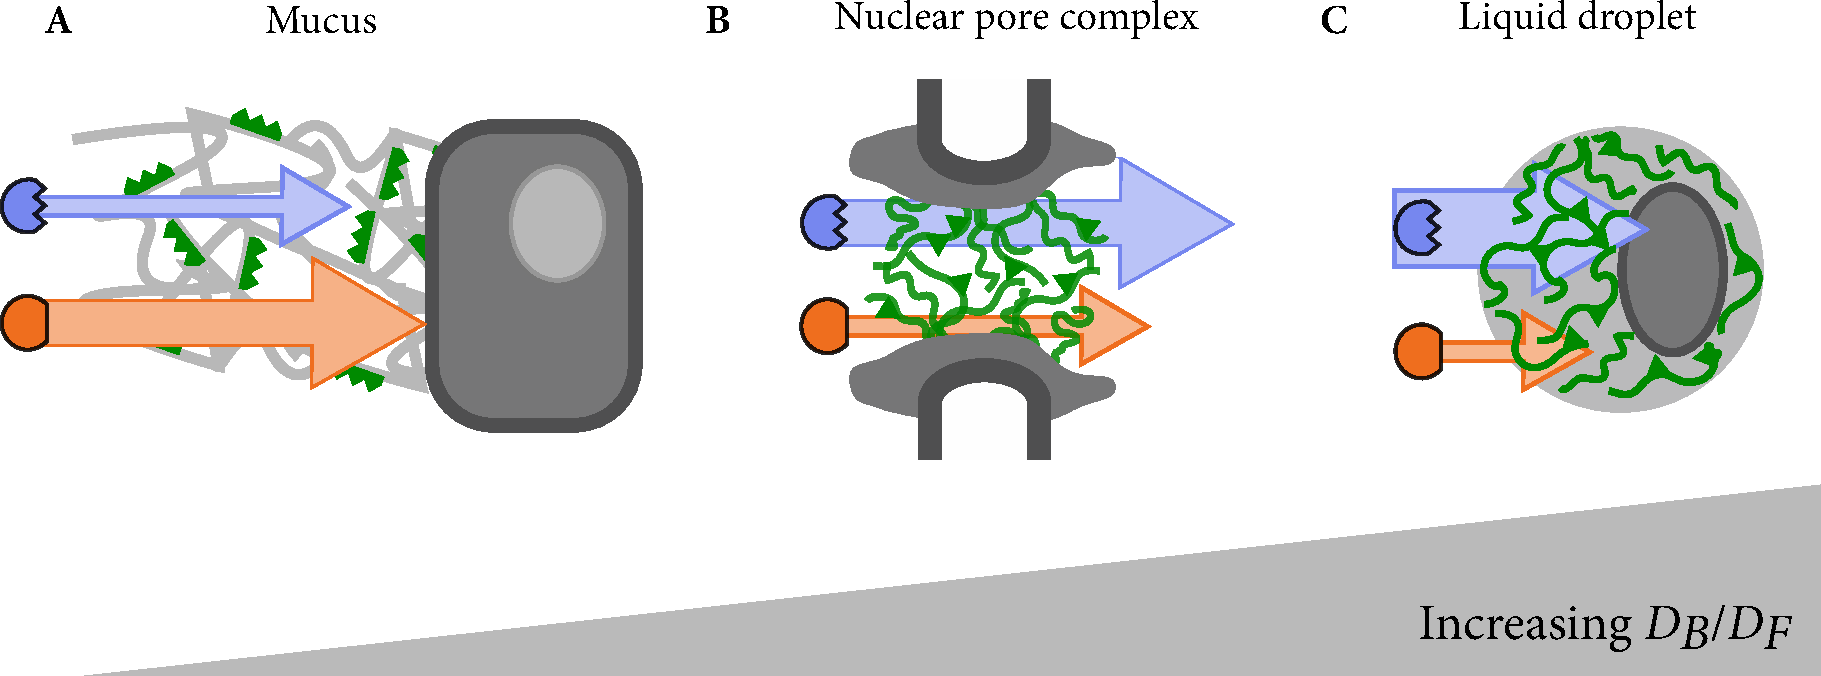
\includegraphics[width=0.8\linewidth]{figs/ch02/concluding-cartoon-large.pdf}
\caption[Bound diffusion in other systems.]{Possible effect of bound diffusion on other biological systems.}
\label{fig:other-filters}
\end{figure}

Systems other than filters may make use of principles found in our model as well.  For example, the bacteria \textit{Staphylococcus aureus}, responsible for many antibiotic-resistant infections in hospitals, can exhibit resistance to the antibiotic vancomycin by constantly building and shedding its cell wall, to which vancomycin binds \cite{mcguinness17}.  Our model predicts that such a strategy should keep the vancomycin flux through the cell wall from reaching steady-state, in the transient regime where the flux of a binding molecule is suppressed (Fig.~\ref{fig:transient}).  The targeting of the DNA damage repair protein PARP1 to appropriate sites in the nucleus, described below, is another potential application of binding and diffusion principles.

\subsection{DNA damage repair protein recruitment in the nucleus}

Poly(ADP-ribose) polymerase 1 (PARP1) is a protein  which assists in DNA damage repair.  Within the nucleus, it rapidly diffuses to and tightly binds damaged DNA, despite the presence of large amounts of undamaged DNA, for which PARP1 also has a measurable affinity \cite{rudolph18,sukhanova16}.  Very little free PARP1 is believed to exist within the nucleus.  Therefore, the rapid migration of PARP1 to damaged DNA must be dependent on bound-state mobility.

Both mechanisms discussed here for the nuclear pore could potentially apply to PARP1 as well.  Johannes Rudoloph, Jyothi Mahadevan, and Karolin Lugar have demonstrated the existence a multivalent``monkey-bar'' mechanism equivalent to inter-chain hopping between DNA strands \cite{rudolph18}.  However, disruption of this mechanism reduces PARP1 diffusion by approximately 10\% only, indicating that there are more methods of bound diffusion available to PARP1 \cite{mahadevan18}

\begin{figure}
\centering
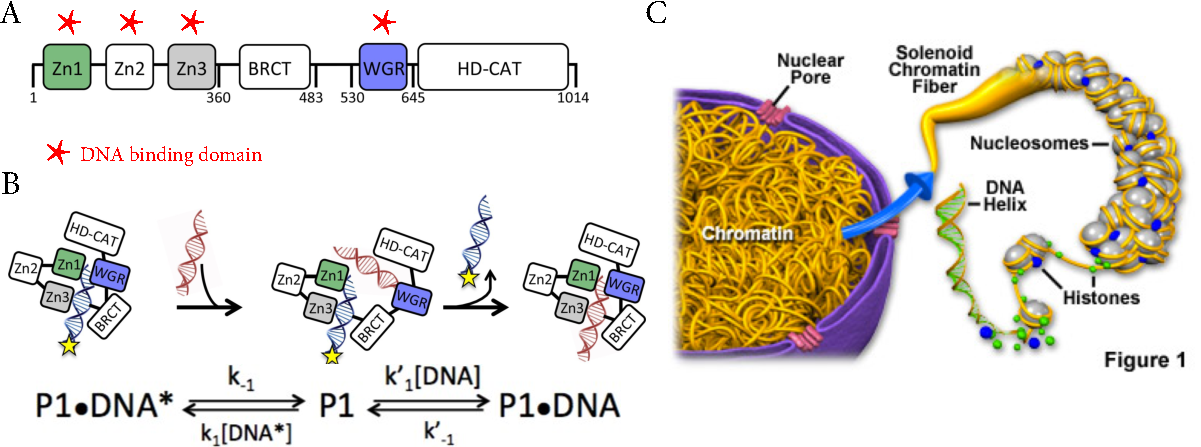
\includegraphics[width=\linewidth]{figs/ch02/PARP1.pdf}
\caption[Possible bound-diffusion mechanisms of PARP1.]{PARP1 and its possible mechanisms of bound diffusion. (A) Schematic of PARP1 structure showing its four DNA-binding domains \cite{rudolph18}. (B) ``Monkey-bar'' inter-strand hopping mechanism cartoon and reaction showing on- and off- rates for binding two subsequent DNA strands \cite{rudolph18}.  (C) Flexible tether structure of chromatin within the nucleus.  (Image from Florida State University.)}
\label{fig:parp1}
\end{figure}

Either tethered diffusion or additional hopping might provide the missing bound-state mobility.  To begin, assume that tethered diffusion is the only additional mechanism of bound diffusion.  The predicted off-rate $\koff$ of PARP1 from undamaged DNA can then be calculated assuming that the effective diffusion constant of PARP1 observed in the nucleus is $D_\mathrm{obs} = p_b D_B + (1-p_b)D_F$, a weighted average of free and bound diffusion constants where $p_b$ is the fraction of PARP1 bound.  If bound diffusion comes only from tethered motion, then $D_B$ is given by Eqn.~\ref{eq:dbound}.  The fraction of PARP1 bound in chemical equilibrium is 
\begin{equation}
p_B = \frac{1}{1+\frac{K_D}{N_T}} 
\end{equation} where $K_D = \koff/\kon$ is the dissociation constant and $N_T$ is the total concentration of PARP1 binding sites on undamaged chromatin (assuming low occupancy by PARP1).

The polymer properties of chromatin are estimated from single-molecule force spectroscopy as $L_c\ell_p = 2.5\times10^{-4}\ \mu$m  - $1.2\times 10^{-5}\ \mu$m \cite{kruithof09, norouzi18}.  Johannes Rudolph estimates a diffusion-limited on-rate of $\kon = 10^{9}\ \mathrm{M}^{-1}\ \mathrm{s}^{-1}$ and a total binding site concentration of up to 1 mM.  Finally, measurements of PARP1 diffusion in the nucleus and in buffer give $D_\mathrm{obs} \approx 3\ \mu\mathrm{m/s}^2$ and an upper bound of $D_F = 9D\mathrm{obs}$ \cite{mahadevan18}.  Using these parameters, we predict that an off-rate between $1.2\times 10^2$ and $1.2\times 10^3\ \mathrm{s}^{-1}$ would account for the observed diffusion.  This off-rate is larger than the commonly accepted range, but not absurd \cite{rudolph18}.

Apart from tethered diffusion, there could be a second mechanism of inter-strand hopping at work.  PARP1 contains four DNA binding domains (Fig.~\ref{fig:parp1}A), and though some may work in tandem, it is possible that additional multivalent interactions are taking place beyond the monkey-bar mechanism.  Analytic models of hopping are more complicated \cite{yang18}, but a highly-simplified model can be used to estimate the maximum expected contribution to bound diffusion from hopping.  Using the reaction scheme described in Fig.~\ref{fig:parp1}B, assume that every time a second strand of DNA binds, PARP1 takes a ``step'' of approximately its own size.  The bound diffusion constant would then be on the order of $D_B \sim R^2 \kon N_T$ where $R$ is the size of PARP1.  Using the parameters above, and taking $R \approx 5$ nm, we have $D_B \approx 1\ \mu\mathrm{m}^2/\mathrm{s}$.  However, given the high concentration of chromatin in the nucleus, the upper bound on bound-state diffusion from hopping can be estimated assuming that there is always a second strand of DNA ``within reach'' of PARP1, i.e. that the binding-site number density is $\rho \approx $ 1 molecule/(5 nm)$^3$.  This assumption leads to a molar concentration [DNA] = 13 mM and a bound diffusion constant $D_B \approx  100\ \mu$m$^2$/s.

Using these order-of-magnitude calculations, either tethered diffusion or hopping could provide enough bound-state mobility to explain the rapid diffusion of PARP1 to sites of DNA damage within the nucleus.

\section{Conclusions}

In the above chapter, we have developed a simple model of selective nuclear transport which may apply more broadly to other biofilters as well.  Remarkably, this simple model can reproduce the high selectivity shown experimentally by the nuclear pore for proteins which can bind to the filter.  The diffusion coefficient of the bound complex proved to be the most important factor in predicting selectivity.  In order to test the predictions of our model, we next began developing nuclear-pore-inspired biofilters to investigate the effect of bound-state diffusion on protein separation \textit{in vitro}.
